\documentclass{article}

\usepackage{fullpage,latexsym,picinpar,amsmath,amsfonts,graphicx}

\input{macros.tex}

\begin{document}
\centerline{REMOVED}
\centerline{REMOVED}
\centerline{\large \bf CS/MATH111 ASSIGNMENT 2}


\vskip 0.1in
%\noindent{\bf Individual assignment:} Problems 1 and 2.

%\noindent{\bf Group assignment:} Problems 1,2 and 3.

\vskip 0.2in


%%%%%%%%%%%%%%%%%%%%%%%%%%%%

\begin{problem}
Alice's RSA public key is $P = (e,n) = (13,77)$.
Bob sends Alice the message by encoding it as follows.
First he assigns numbers to characters:
A is 2, B is 3, ..., Z is 27, and blank is 28. Then he
uses RSA to encode each number separately. 

Bob's encoded message is:

\begin{verbatim}
     10       7      58      30      23      62 
      7      64      62      23      62      61 
      7      41      62      21       7      49 
     75       7      69      53      58      37 
     37      41      10      64      50       7 
     10      64      21      62      61      35 
     62      61      62       7      52      10 
     21      58       7      49      75       7 
     62      26      22      53      30      21 
     10      37      64
\end{verbatim}

Decode Bob's message.
Notice that you don't have Bob's secrete key, so you
need to ``break" RSA to decrypt his message.

\smallskip
For the solution, you need to provide the following:
%
\begin{itemize}
%
\item Describe step by step how you arrived at the solution.
	In particular, explain how you determined $p$, $q$, $\phi(n)$, and $d$.
%
\item Show the calculation that determines the first three letters in the message from the first three numbers in ciphertext.
%
\item Give Bob's message in plaintext. The message is a quote. Who said it? What does it mean?
%
\item If you wrote a program, attach your code to the hard copy.
	If you solved it by hand (not recommended), attach your scratch paper with calculations
	for at least 5 first letters.
%
\end{itemize}

Suggestion: this can be solved by hand, but it will probably
be faster to write a short program.
\end{problem}

\begin{solution}
First, we will need to solve for what the secret RSA key is that Bob has.

This is done through guessing factorization of $n$.

$P=(e, n) = (13, 77)$

The only primes that go into 77 are $7\cdot11$. 
\newline

$p=7$ and $q = 11$.
\newline

Now that we have this information, we plug in $p$ and $q$ into Euler's Totient Algorithm.
\newline
$φ(n) = (p-1)(q-1) = (7-1)(11-1) = 6\cdot10 = 60$
\newline

The secret key of variable $d$ is found through the following formula:
\newline
$d = e^{-1}(mod(n))$ = $d=13^{-1}(mod(60))$
\newline

We now find the LCD of 13 and $60+1$. We have a list of common multiples starting at 61 and adding 60 after each:
\newline

61, 121, 181, 241, 301, 361, 421, 481
\newline

13 goes into 481 37 times.
\newline

Therefore, $d=37$.

Now that we have our decryption $d$ of 37, we can plug it into the decryption private key pair, which is $(d, n)$. We plug in 37 for $d$ and 77 for $n$.
\newline

We now use the following formula to decrypt Bob's message characters:
\newline
$M = C^{d} (mod(n))$
\newline

$C$ is the variable that the encoded character is put into the formula.
\newline

$M = C^{37} \cdot mod(77)$
\newline

To solve for the first letter, we do the following:

The encoded character is 10.
\newline
10^{d}\pmod{n} = 10^{37}\pmod{77} \\
= (10^2)^{18}\cdot 10\pmod{77} = 23^{18}\cdot 10\pmod{77} \\
= (23^2)^{9}\cdot 10\pmod{77} = 67^9\cdot 10\pmod{77} \\
= (67^2)^{4}\cdot 67\cdot 10\pmod{77} = 23^4\cdot 67\cdot 10\pmod{77} \\ 
= (23^2)^{2}\cdot 670\pmod{77} = 67^2\cdot 670\pmod{77} \\ 
= 23\cdot 670\pmod{77} = 15,410\pmod{77} = 10 \\ 
\newline
\textrm{We have successfully decoded the character as 10, which is the letter "I"}
\newline


To solve for the second letter, we do the following:

The encoded character is 7.
\newline
7^{d}\pmod{n} = 7^{37}\pmod{77} \\
= (7^2)^{18}\cdot 7\pmod{77} = 49^{18}\cdot 7\pmod{77} \\
= (49^2)^{9}\cdot 7\pmod{77} = 14^9\cdot 7\pmod{77} \\
= (14^2)^{4}\cdot 14\cdot 7\pmod{77} = 42^4\cdot 14\cdot 7\pmod{77} \\ 
= (42^2)^{2}\cdot 98\pmod{77} = 70^2\cdot 98\pmod{77} \\ 
= 49\cdot 98\pmod{77} = 4,802\pmod{77} = 28 \\ 
\newline
\textrm{We have successfully decoded the character as 28, which is a blank space}
\newline

To solve for the third letter, we do the following:

The encoded character is 58.
\newline
58^{d}\pmod{n} = 58^{37}\pmod{77} \\
= (58^2)^{18}\cdot 58\pmod{77} = 53^{18}\cdot 58\pmod{77} \\
= (53^2)^{9}\cdot 58\pmod{77} = 37^9\cdot 58\pmod{77} \\
= (37^2)^{4}\cdot 37\cdot 58\pmod{77} = 60^4\cdot 37\cdot 58\pmod{77} \\ 
= (60^2)^{2}\cdot 2,146\pmod{77} = 58^2\cdot 2,146\pmod{77} \\ 
= 53\cdot 2,146\pmod{77} = 113,738\pmod{77} = 9 \\ 
\newline
\textrm{We have successfully decoded the character as 9, which is the letter "H"}
\newline

Once the code has executed, the output is the following: 
\newline
"I HAVE NEVER LET MY SCHOOLING INTERFERE WITH MY EDUCATION".
This quote is by Mark Twain.
\newline
The code that outputted the rest is the following:
\begin{center}
		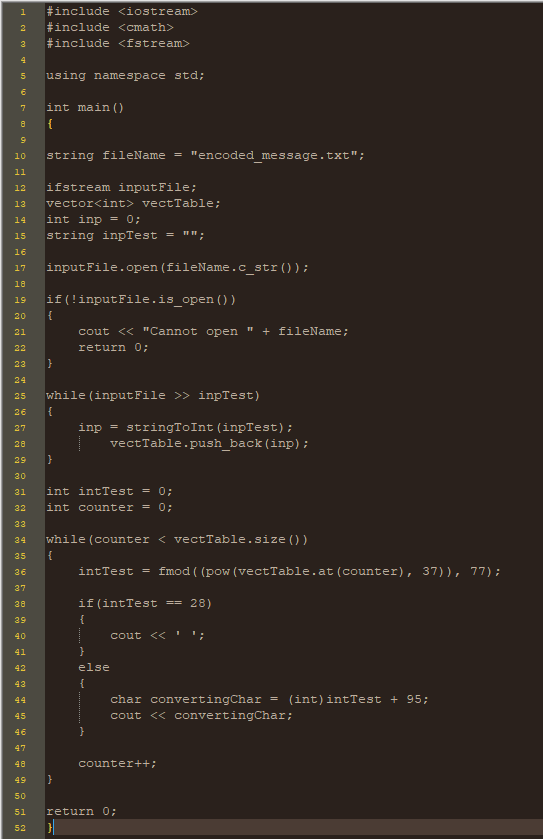
\includegraphics{files/codeblock.PNG}
\end{center}

\newline

\end{solution}

%%%%%%%%%%%%%%%%%%%%%%%%%%%%
\bigskip
\begin{problem}
(a) Compute $13^{-1}\pmod{19}$ by enumerating multiples of the number and the modulus.
Show your work.

\smallskip\noindent
(b) Compute $13^{-1}\pmod{19}$ using Fermat's theorem. Show your work.

\smallskip\noindent
(c) Compute $13^{-40}\pmod{19}$ using Fermat's theorem. Show your work.

\smallskip\noindent
(d) Find a number $x\in\braced{1,2,...,36}$
	such that $8x \equiv 3 \pmod{37}$. Show your work.
	(You need to follow the method covered in class; brute-force checking
	all values of $x$ will not be accepted.)
\end{problem}

\begin{solution}
\\\\(a)
\\ $13^{-1}(mod (19))$
\\ $13a = 19b + 1$
\\\\ The GCD of these numbers is 1 as they are co-prime
\\\\ This means that the LCM $ = 13*19 = 247$
\\\\ This gives a formula of:
\\ $19*13 = 1(mod(19))$
\\\\ As $a = 19$ and $b = 13$
\\\\ This can then be combined with the original problem:
\\ $13^{-1} = 19(mod(19))$
\\\\ Which is equivalent to zero.
\\\\ Therefore:
\\ $13^{-1}(mod (19)) = 0$
\newline
\\\\ (b)
\\ $13^{-1}(mod (19))$ using FLT
\\ FLT: $a^p = a(mod(p))$
\\ $13^8 = 1(mod(19))$
\\ $13^{-1}(13^{18})(mod(19)) = 13^{17}(mod(19))$
\\ $13^{17}(mod(19)) = $
\\ $13^813^9(mod(19)) = $
\\ $13^413^413^413^413(mod(19))$
\\ $13^4(mod(19)) = 4$
\\ $13(mod(19)) = 13$
\\\\ The solved values can then be combined into a simpler problem:
\\ $(4*4*4*4*13)(mod(19)) = $
\\ $3328(mod(19)) = 3$
\\\\\ Therefore:
\\ $13^{-1}(mod (19)) = 3$
\newline
\\\\ (c)
\\ $13^{-40}(mod (19))$
\\\\ Using FLT:
\\ $13^{18} = 1 (mod (19))$
\\\\ Combine with problem:
\\ $13^{-40}13^{18} = 1(mod (19))$
\\\\ Repeat:
\\ $13^{-22}13^{18} = 1(mod (19))$
\\\\ Repeat:
\\ $13^{-4}13^{18} = 1(mod (19))$
\\\\ In solvable form:
\\ $13^{14}(mod (19))$
\\ $13^813^6(mod (19))$
\\ $13^413^413^213^213^2(mod (19))$
\\ $13^4(mod (19)) = 4$
\\ $13^2(mod (19)) = 17$
\\ $(4*4*17*17*17)(mod (19)) = $
\\ $78,608(mod (19)) = 5$
\\\\ Therefore:
\\ $13^{-40}(mod (19)) = 5$
\newline
\\\\ (d)
\\ $8x = 3(mod (37))$
\\ $8*a = 37*b+3$
\\ First find the LCM:
\\ $40*1, 8*5$
\\\\ Then put these numbers into the above altered equation: 
\\ $8(5) = 3(mod(37))$
\\\\ Therefore by looking at this equation:
\\ $x = 5$

\end{solution}

%%%%%%%%%%%%%%%%%%%%%%%%%%%%

\vskip 0.1in



%%%%%%%%%%%%%%%%%%%%%%%%%%%%%%%%%%%%%%%%%%%%%%%%%%%%%%%%%%%%%%%%%%%%%
\begin{problem}
Strings of length $n$ are composed of the following strings: $\tt1$, $\tt2\tt2$, $\tt2\tt3$, $\tt3\tt2$, $\tt3\tt3$,
$\tt4\tt4\tt5$ and $\tt5\tt4\tt4$. Let $S_n$ be the number of strings of length $n$ that can
be formed in this way. For example, for $n=3$, we can form the following strings:
%
\begin{align*}
\tt1\tt1\tt1
,
\tt1\tt2\tt2  , \tt1\tt2\tt3  , \tt1\tt3\tt2  , \tt1\tt3\tt3
,
\tt2\tt2\tt1  , \tt2\tt3\tt1  , \tt3\tt2\tt1  , \tt3\tt3\tt1 
,
\tt4\tt4\tt5 , \tt5\tt4\tt4
\end{align*}
%
and thus $S_3 = 11$. (Note that $S_0 = 1$, because the
empty string satisfies the condition.)

\smallskip
\noindent (a) Derive a recurrence relation for the numbers $S_n$. Justify it.

\smallskip
\noindent (b) \textbf{Extra credit}. Let $P_n$ be the number of strings of length $n$ that can
be formed from the given strings,  considering that four 1's cannot be next to each other. (The substring 1111 is not allowed.) Derive a recurrence relation for the numbers $P_n$. Justify it.
\smallskip

%\noindent (b) Find the formula for the numbers $S_n$ by solving this recurrence. Show your work.
\end{problem}
\newline

\begin{solution}
\\\\ (a)
\\\\ Given: $S_3 = 11, S_0 = 1$
\newline
$S_1 = 1$ We only have a single string character here.
\newline
$S_2 = 5$ We have the single string character, followed by a total of four 2 string characters.
\newline
\\\\ Therefore:
\\ $S_{n-1} $ has a coefficient of 1
\\ $S_{n-2}$ has combos of: 
\\ $22, 23, 11$
\newline
\\ Therefore $S_{n-2}$ has a coefficient of 3
\\ $S_{n-3}$ has a coefficient of 11
\newline

Therefore, we derive the recurrence relation of:
$ S_{n} = S_{n-3} + S_{n-3} + 2S_{n-2} + 2S_{n-2} + S_{n-1} $
\newline

This simplifies to:
$S_{n} = 2S_{n-3} + 4S_{n-2} + S_{n-1}$
\newline

\\\\ (b)
\\\\As this string is four characters long, $S_{n-4}$ is affected.
\\\\In order to satisfy the requirement of not having 1111 next to each other, we have to subtract that value from $S_{n-4}$. So, the solution would be:
\newline
$P_n=S_{n-3} + 3S_{n-2} + S_{n-1} - 62S_{n-4}$
\\\\ As the substrings of 111, 11 and 1 would have to be removed as well as there would be the possibility that they would be the end of a 1111 string.

\end{solution}

\smallskip
%%%%%%%%%%%%%%%%%%%%%%%%%%%%

\begin{problem}
Solve the following recurrence equation:
\smallskip
\begin{align*}
	S_n &= S_{n-1} + 4S_{n-2} + 2S_{n-3}
	\\
	S_0 &= 1
	\\
	S_1 &= 1
	\\
	S_2 &= 5
\end{align*}

\noindent Show your work (all steps: the characteristic polynomial and its roots, the general solution, 
using the initial conditions to compute the final solution.)
\end{problem}

\large
\begin{solution}
\\S_n - S_{n-1} - 4S_{n-2} - 2S_{n-3} = 0
\newline
\\r^3-r^2-4r-2=0
\newline
\\(r+1)(r^2-2r-2)
\newline
\\\\ $Via quadratic formula:$
\newline
\\x = \frac{-b+-\sqrt{b^2*4a}}{2a}
\newline
\\x=\frac{2+-\sqrt{12}}{2}=
\\x=\frac{2+-2\sqrt{3}}{2}=
\\x=1+-\sqrt{3}
\newline
\\\\ $Therefore the roots of the equation are:$
\\(r+1)(r+1+\sqrt{3})(x+1-\sqrt{3})
\newline
\\\\ $This gives a general formula of:$
\\a_n = \alpha_1(-1)^n+\alpha(1-\sqrt{3})^n+\alpha(1+\sqrt{3})^n
\\\\$The initial values can then be used here:$
\newline
\\a_0=\alpha_1(-1)^0+\alpha_2(1-\sqrt{3})^0+\alpha_3(1+\sqrt{3})^0
\\a_0=\alpha_1+\alpha_2+\alpha_3 = 1
\newline
\\a_1=\alpha_1(-1)^1+\alpha_2(1-\sqrt{3})^1+\alpha_3(1+\sqrt{3})^1
\\a_1=-\alpha_1+(1-\sqrt{3})\alpha_2+(1-\sqrt{3})\alpha_3 = 5
\newline
\\a_2 = \alpha_1(-1)^2+\alpha_2(1-\sqrt{3})^2+\alpha_3(1+\sqrt{3})^2
\\a_2 = \alpha_1+(4-2\sqrt{3})\alpha_2+(4+2\sqrt{3})\alpha_3 = 5
\newline
\\\\ $These can then be used to create a system of equations to solve for the $ \alpha $s$
\\\\ $For the sake of simplicity and to increase ease of understanding the values x, y, and z will be used in place of the $ \alpha $s in the order of 1, 2, 3 only for the system of equations explanation: $
\\\\ $First rearrange the simplest equation to solve for x as that will be needed: $
\\ $x = 1 - y - z$
\newline
\\\\ $This can then be plugged in as x in the other two equations: $
\\ $-(1-y-z)+(1-\sqrt{3})y+(1+\sqrt{3})z = 1$
\\ $1-y-z+(4-2\sqrt{3})y+(4+2\sqrt{3})z = 5$
\newline
\\\\ Next move the variables around to get y alone on one side: 
\\ $-(1-y-z)+(1-\sqrt{3})y+(1+\sqrt{3})z -(1+\sqrt{3})z = 1 - (1+\sqrt{3})z$
\\ $-(1-y-z) + (1-\sqrt{3})y = 1 - (1+\sqrt{3})z$
\\ $-1+y+z + (1-\sqrt{3})y = 1 - (1+\sqrt{3})z$
\\ $2y - \sqrt{3}y + z - 1 = 1 - (1+\sqrt{3})z$
\\ $2y - \sqrt{3}y -1 = 1 - (1+\sqrt{3})z - z$
\\ $2y - \sqrt{3} -1 +1 = -2z-\sqrt{3z}+2$
\\ $2y -\sqrt{3}y = -2z-\sqrt{3}z+2$
\\ $y(2-\sqrt{3}) = -2z-\sqrt{3}z+2$
\\ $y = (2+\sqrt{3})(-2z-\sqrt{3}z+2)$
\newline
\\\\ This can then be substituted in:
\\ $1-(2+\sqrt{3})(-2z-\sqrt{3}z+2)-z+(4-2\sqrt{3})(2+\sqrt{3})(-2z-\sqrt{3}+2)(4+2\sqrt{3})z = 5$
\newline
\\\\ Then z can be solved for:
\\ $-(2+\sqrt{3})(-2z-\sqrt{3}z+2)-z+(4-2\sqrt{3})(2+\sqrt{3})(-2z-\sqrt{3}+2)(4+2\sqrt{3})z = 4$
\newline
\\\\ Simplified pieces:
\\ $-(2+\sqrt{3})(-2z-\sqrt{3}z+2) = $
\\ $(-2-\sqrt{3})(-2z-\sqrt{3}z+2) = $
\\ $7z+4\sqrt{3}z-4-2\sqrt{3}$
\newline
\\ $(4-2\sqrt{3})(2+\sqrt{3})(-2z-\sqrt{3}z+2) = $
\\ $-4z-2\sqrt{3z+4}$
\\\\ Combine simplified forms:
\\ $7z+4\sqrt{3}z-4-2\sqrt{3}-z-4z-2\sqrt{3}z+4+4z+2\sqrt{3}z = $
\\ $6z+4\sqrt{3}z-2 = 4$
\newline
\\\\ Add $2\sqrt{3}$ to both sides and simplify:
\\ $6z+4\sqrt{3}z = 4 + 2\sqrt{3}$
\\ $2(3+2\sqrt{3})z = 4+2\sqrt{3}$
\\ $z = \frac{4+2\sqrt{3}}{2(3+2\sqrt{3})}$
\\ $z = \frac{2(2+\sqrt{3})}{2(3+2\sqrt{3})}$
\newline
\\\\ Reduce z down to the simplest form possible:
\\ $z = \frac{2+\sqrt{3}}{3+2\sqrt{3}}$
\\ $z = \frac{2+\sqrt{3}}{\sqrt{3}(\sqrt{3}+2)}$
\\ $z = \frac{1}{\sqrt{3}}$
\newline
\\\\ Rationalize:
\\ $z = \frac{\sqrt{3}}{3}$
\newline
\\\\ As z has been found it can be plugged in to find y:
\\ $y = (2+\sqrt{3})(-2(\frac{\sqrt{3}}{3})-\sqrt{3}(\frac{\sqrt{3}}{3})+2)$
\\ $y = (2+\sqrt{3})(\frac{-2}{\sqrt{3}}+1)$
\\ $y = 2(\frac{-2}{\sqrt{3}}) + 2(1+\sqrt{3}(\frac{-2}{\sqrt{3}}))+\sqrt{3}$
\\ $y = \frac{-4}{\sqrt{3}}+2(1-\frac{\sqrt{3}*2}{\sqrt{3}}+\sqrt{3})$
\\ $y = \frac{-4}{\sqrt{3}}+\sqrt{3}$
\\ $y = \frac{-4\sqrt{3}}{3}+\sqrt{3}$
\newline
\\\\ As y has been found it can be plugged in to solve for x:
\\ $x = 1 - (\frac{-4\sqrt{3}}{3}+\sqrt{3})-\frac{\sqrt{3}}{3}$
\\ $x = 1 + \frac{4}{\sqrt{3}}-\sqrt{3}-\frac{\sqrt{3}}{3}$
\\ $x = 1+ \frac{4}{\sqrt{3}} - \sqrt{3} - \frac{1}{\sqrt{3}}$
\\ $x = \frac{4}{\sqrt{3}}-\frac{1}{\sqrt{3}}+1-\sqrt{3}$
\\ $x = \sqrt{3}+1-\sqrt{3}$
\\ $ x = 1$
\newline
\\\\ These are the values of $\alpha$ :
\\ $\alpha_1 = 1$
\\ $ \alpha_2 = \frac{-4\sqrt{3}}{3}+\sqrt{3} = \frac{\sqrt{3}}{3}$
\\ $\alpha_3 = \frac{\sqrt{3}}{3}$
\newline
\\\\ These values can be plugged into the general formula to get the final solution:
\\ $a_n = (-1)^n+(-\frac{\sqrt{3}}{3})(1-\sqrt{3})^n+(\frac{\sqrt{3}}{3})(1+\sqrt{3})^n$




\end{solution}


\end{document}

